\documentclass[a4paper]{article}
\usepackage[utf8]{inputenc}
\usepackage{amsmath}
\usepackage{amssymb}
\usepackage{mathtools}
\usepackage{amsfonts}
\usepackage{lastpage}
\usepackage{tikz}
\usepackage{float}
\usepackage{textcomp}
\usetikzlibrary{patterns}
\usepackage{pdfpages}
\usepackage{gauss}
\usepackage{fancyvrb}
\usepackage[table]{colortbl}
\usepackage{fancyhdr}
\usepackage{graphicx}
\usepackage[margin=2.5 cm]{geometry}

\definecolor{listinggray}{gray}{0.9}
\usepackage{listings}
\lstset{
	language=,
	literate=
		{æ}{{\ae}}1
		{ø}{{\o}}1
		{å}{{\aa}}1
		{Æ}{{\AE}}1
		{Ø}{{\O}}1
		{Å}{{\AA}}1,
	backgroundcolor=\color{listinggray},
	tabsize=3,
	rulecolor=,
	basicstyle=\scriptsize,
	upquote=true,
	aboveskip={0.2\baselineskip},
	columns=fixed,
	showstringspaces=false,
	extendedchars=true,
	breaklines=true,
	prebreak =\raisebox{0ex}[0ex][0ex]{\ensuremath{\hookleftarrow}},
	frame=single,
	showtabs=false,
	showspaces=false,
	showlines=true,
	showstringspaces=false,
	identifierstyle=\ttfamily,
	keywordstyle=\color[rgb]{0,0,1},
	commentstyle=\color[rgb]{0.133,0.545,0.133},
	stringstyle=\color[rgb]{0.627,0.126,0.941},
  moredelim=**[is][\color{blue}]{@}{@},
}

\lstdefinestyle{base}{
  emptylines=1,
  breaklines=true,
  basicstyle=\ttfamily\color{black},
}

\pagestyle{fancy}
\def\checkmark{\tikz\fill[scale=0.4](0,.35) -- (.25,0) -- (1,.7) -- (.25,.15) -- cycle;}
\newcommand*\circled[1]{\tikz[baseline=(char.base)]{
            \node[shape=circle,draw,inner sep=2pt] (char) {#1};}}
\newcommand*\squared[1]{%
  \tikz[baseline=(R.base)]\node[draw,rectangle,inner sep=0.5pt](R) {#1};\!}
\cfoot{Page \thepage\ of \pageref{LastPage}}
\DeclareGraphicsExtensions{.pdf,.png,.jpg}
\author{Nikolaj Dybdahl Rathcke (rfq695)}
\title{Fourth Home Assignment \\ Data Analysis}
\lhead{Nikolaj Dybdahl Rathcke (rfq695)}
\chead{Data Analysis}
\rhead{Assignment 4}

\begin{document}
\maketitle
\section*{Question 1}
\subsection*{(1)}
We want to prove that
\begin{align}
\mathbb{E}[X+Y]=\mathbb{E}[X]+\mathbb{E}[Y]
\label{q1_1a}
\end{align}
We know that from definition that
$$\mathbb{E}[X]=\sum_{x\in \mathcal{X}}xp_X(x)$$
This means we can write
\begin{align*}
\mathbb{E}[X+Y] &=\sum_{x\in \mathcal{X}}\sum_{y\in \mathcal{Y}} (x+y)p_{XY}(x,y)\\
                &= \sum_{x\in \mathcal{X}}x\sum_{y\in \mathcal{Y}} p_{XY}(x,y)+ \sum_{y\in \mathcal{Y}}y\sum_{\in \mathcal{X}} p_{XY}(x,y)\\
                &= \sum_{x\in \mathcal{X}}xp(x)+\sum_{y\in \mathcal{Y}}yp(y) \\
                &= \mathbb{E}[X]+\mathbb{E}[Y]
\end{align*}
Which means we have proven equation \ref{q1_1a}.
\subsection*{(2)}
We want to show, when $X$ and $Y$ are independent, then
\begin{align}
\mathbb{E}[XY]=\mathbb{E}[X]\mathbb{E}[Y]
\label{q1_2a}
\end{align}
We have the following definition
$$\mathbb{E}[X]=\sum_{x\in \mathcal{X}}xp_X(x)$$
This means we can write the following
\begin{align*}
\mathbb{E}[XY]           &= \sum_{x\in \mathcal{X}}\sum_{y\in \mathcal{Y}} xy p_{XY}(x,y)\\
&= \sum_{x\in \mathcal{X}}\sum_{y\in \mathcal{Y}} xyp_{X}(x)p_{Y}(y) &\rightarrow\mbox{using independence assumption} \\
                         &= \sum_{x\in \mathcal{X}}xp_{X}(x)\sum_{y\in \mathcal{Y}} yp_{Y}(y) \\
                         &= \mathbb{E}[X]\mathbb{E}[Y]
\end{align*}
which proves equation \ref{q1_2a}.

\subsection*{(3)}
As an example, let $X$ and $Y$ be two cards drawn from the same standard deck of cards (without replacement).\\
In this example, for both $X$ and $Y$ then $\mathbb{E}\{\mbox{card is red}\}=\mathbb{E}\{\mbox{card is black}\}=\frac{1}{2}$.\\
The joint distribution of $X$ and $Y$ is
\begin{center}
\begin{tabular}{c||c|c}
X\textbackslash Y & R & B \\
\hline
\hline
R & 25/102  & 26/102 \\
\hline
B & 26/102 & 25/102 \\
\end{tabular}
\end{center}
We get that
\begin{align*}
\mathbb{E}[X=R,Y=R]&=25/102 \\
\mathbb{E}[X=R]\mathbb{E}[Y=R]&=1/2\cdot 1/2 = 1/4
\end{align*}
which means
\begin{align*}
\mathbb{E}[XY]\neq \mathbb{E}[X]\mathbb{E}[Y]
\end{align*}
because the random variables are not independent of eachother.

\subsection*{(4)}
We want to prove
\begin{align}
\mathbb{E}[\mathbb{E}[X]]=\mathbb{E}[X]
\label{q1_4a}
\end{align}
The expected value of a random variable will be just some constant $c$. So $\mathbb{E}[X]=c$. An expected value of a constant is the constant itself, so $\mathbb{E}[c]=c$, thus we get
\begin{align*}
\mathbb{E}[\mathbb{E}[X]]&=\mathbb{E}[c] \\
&= c
\end{align*}
which proves equation \ref{q1_4a}.

\newpage
\section*{Question 2}
\subsection*{(1)}
We want to show that
\begin{align}
\mathbb{P}\{\mbox{$N$ green balls are pulled in a row}\}\leq e^{-N\varepsilon}
\label{q2_1a}
\end{align}
The probability of pulling $N$ green balls out in a row is the same as the chance of not drawing red balls $N$ times. The probability of drawing a red ball when there are $2N$ balls is $2N\varepsilon/2N$, thus the chance of drawing a green ball is $1-(2N\varepsilon/2N)$. Since we are not replacing the balls, the probability for drawing a red ball increases each time we pull out a green one because the total number of balls decreases and so does the number of green ones. It can be expressed as
\begin{align*}
\prod_{i=0}^{N-1} \left(1-\frac{2N\varepsilon}{2N-i}\right)
\end{align*}
We can rewrite equation \ref{q2_1a}
\begin{align*}
\prod_{i=0}^{N-1} \left(1-\frac{2N\varepsilon}{2N-i}\right) &\leq e^{-N\varepsilon}
\end{align*}
We use the inequality $1+x\leq e^x$ to get
\begin{align*}
\prod_{i=0}^{N-1} \left(1-\frac{2N\varepsilon}{2N-i}\right) &\leq \prod_{i=0}^{N-1} e^{-\frac{2N\varepsilon}{2N-i}} \\
&= e^{\sum_{i=0}^{N-1}-\frac{2N\varepsilon}{2N-i}} \\
&= e^{-2N\varepsilon\sum_{i=0}^{N-1}\frac{1}{2N-i}}
\end{align*}
The sum will always provide values in $[\frac{1}{2}, 1)$. This means that
\begin{align*}
\mathbb{P}\{\mbox{$N$ green balls are pulled in a row}\}\leq e^{-2N\varepsilon\sum_{i=0}^{N-1}\frac{1}{2N-i}}\leq e^{-2N\varepsilon}\leq e^{-N\varepsilon}
\end{align*}
And thus, equation \ref{q2_1a} is shown.

\newpage
\section*{Question 3}
\subsection*{(1)}
We want to prove that
\begin{align}
m_{\mathcal{H}}(2N)\leq m_{\mathcal{H}}(N)^2
\label{q3_1a}
\end{align}
We let
\begin{align}\label{q3_1b}
m_{\mathcal{H}}(N)= c
\end{align}
If we partition a set of $2N$ points into sets of $N$ points, then that means we get $c$ dichotomies in each of these sets. These two sets can, at maximum produce dichotomies corresponding to the cross product of the two sets of dichotomies. That means the LHS of equation \ref{q3_1a} has the upper bound
\begin{align*}
m_{\mathcal{H}}(2N)&\leq c\cdot c \\
&=c^2 \\
&=m_{\mathcal{H}}(N)^2
\end{align*}
Last step using equation \ref{q3_1b}, and thus equation \ref{q3_1a} is proved.

\subsection*{(2)}
Equation 2.12 in [LFD] states that
\begin{align*}
E_{out}(g)\leq E_{in}(g)+\sqrt{\frac{8}{N}\ln \frac{4m_{\mathcal{H}}(2N)}{\delta}}
\end{align*}
Substituting the upper bound we found in (1) for $m_\mathcal{H}(2N)$, we can write a generalization bound that does not include this factor
\begin{align*}
E_{out}(g)\leq E_{in}(g)+\sqrt{\frac{8}{N}\ln \frac{4m_{\mathcal{H}}(N)^2}{\delta}}
\end{align*}
This upper bound is a bit looser.

\newpage
\section*{Question 4}
\subsection*{(1)}
We want to prove that
\begin{align}
\sum_{i=0}^d\binom{N}{i}&\leq N^d+1
\label{q4_1a}
\end{align}
when $d\leq N$
We begin by setting $d=0$ and get
\begin{align*}
\sum_{i=0}^0\binom{N}{i}&\leq N^0+1 &\Leftrightarrow \\
1&\leq1+1
\end{align*}
which holds. Now we do our induction step, assuming equation \ref{q4_1a} (hypothesis) holds for $d$ we want to prove that it holds for $d+1$
\begin{align*}
\sum_{i=0}^{d+1}\binom{N}{i}&\leq N^{d+1}+1
\end{align*}
for $d\geq 1$. We can rewrite this to
\begin{align*}
\sum_{i=0}^{d}\binom{N}{i}+\binom{N}{d+1}&\leq N^{d+1}+1 \\
&=N^d+(N-1)N^d+1
\end{align*}
Using our hypothesis we can write
\begin{align*}
N^d+1+\binom{N}{d+1}&\leq N^d+(N-1)N^d+1 &\Leftrightarrow \\
\binom{N}{d+1}&\leq (N-1)N^d
\end{align*}
The right hand side will always be larger since we are only looking at $d\geq 1$. Therefore equation \ref{q4_1a} holds.

\subsection*{(2)}
From [LFD] equation (2.9):
\begin{align*}
m_\mathcal{H}(N)\leq \sum_{i=0}^d \binom{N}{i}
\end{align*}
This means we can derive the following bound
\begin{align*}
m_\mathcal{H}(N)\leq N^d+1
\end{align*}
using our result from (1).

\subsection*{(3)}
Equation 2.12 in [LFD]:
\begin{align*}
E_{out}(g)\leq E_{in}(g)+\sqrt{\frac{8}{N}\ln \frac{4m_{\mathcal{H}}(2N)}{\delta}}
\end{align*}
Substituting the result in the equation yields
\begin{align*}
E_{out}(g)\leq E_{in}(g)+\sqrt{\frac{8}{N}\ln \frac{4(2N)^d+1)}{\delta}}
\end{align*}
The coefficient $d$ should be relatively small compared to $N$ so the bound is not too loose. The smaller $d$ compared to $N$, the tighter the bound.

\newpage
\section*{Question 5}
\subsection*{(1)}
We implement $k$-means clustering in Matlab, one thing differing to the standard implementation of this is that, instead of seeing if the centroids are exactly alike, we see if the sum of their differences is sufficiently small $> 0.001$, seeing if the centroids have changed by doing a comparison will fail due to rounding errors.
\\
This is applied to the first 100 instances of each digit in the MNINST training set, we set $k = 2$ to find two clusters as specified. Now a plot of $E_{in}$ as a a funtion of the number of iterations of the k-means algorithm, this plot can be seen in figure \ref{opg51}.
\begin{figure}[H]
  \centering
  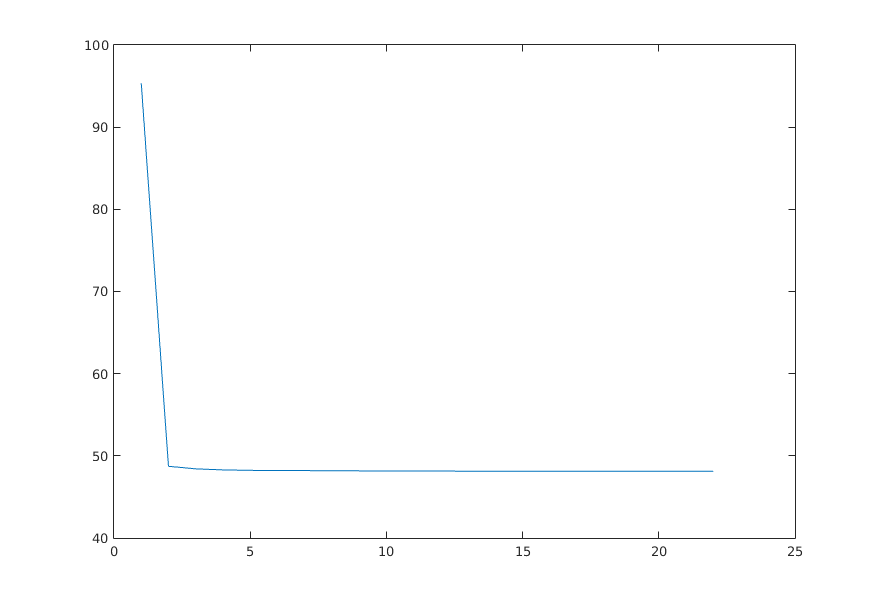
\includegraphics[width=\textwidth]{./51.png}
  \caption{}
  \label{opg51}
\end{figure}
It is verified that $E_{in}$ monotonically decreases, thus the algorithm is not obviously faulty implemented.
\newpage
\subsection*{(2)}
The same experiment is done with $k=4$, the plot for this can be seen in figure \ref{opg52}.
\begin{figure}[H]
  \centering
  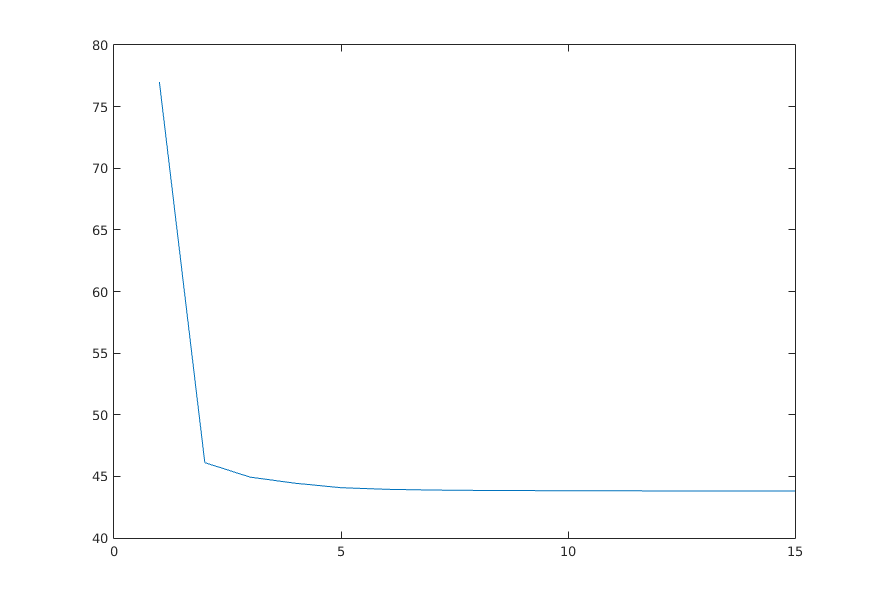
\includegraphics[width=\textwidth]{./52.png}
  \caption{}
  \label{opg52}
\end{figure}
\subsection*{(3-4)}
k-means is now applied to cluster the dataset into $k =[2,3,4,5,6,7,8,9,10,11,12,13,14,15,16]$ clusters, for each $k$ we apply 5 random initializations of the algorithm and pick the best outcome.

\newpage
\subsection*{(5)}
For the data calculated in (3-4) we plot $E_{in}$ as a function of k. This plot can be seen below in figure \ref{opg55}.
\begin{figure}[H]
  \centering
  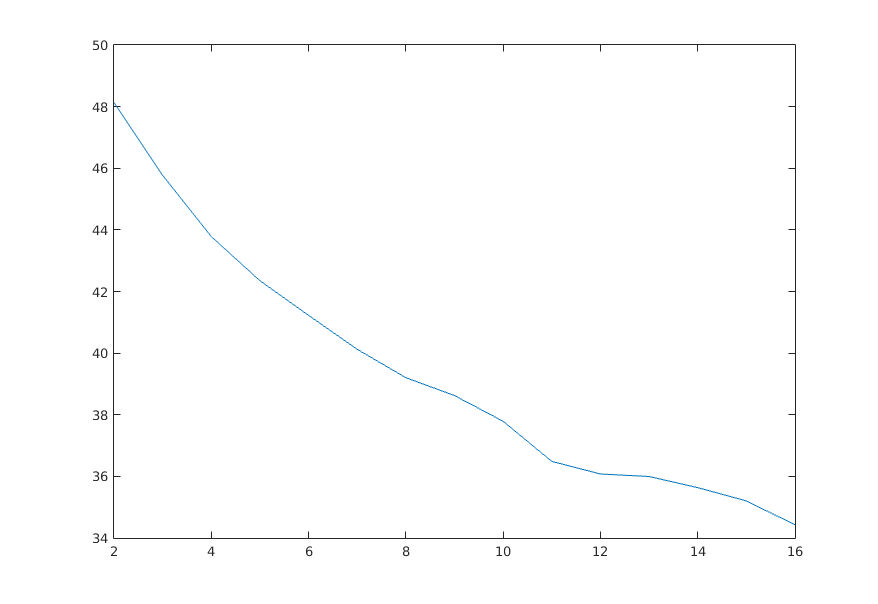
\includegraphics[width=\textwidth]{./55.png}
  \caption{}
  \label{opg55}
\end{figure}
It can easily be seen that $E_{in}$ monotonically decreases, this makes sense as the more clusters we have the smaller distance there will be to their closest centroid.

\newpage
\subsection*{(6)}
For $k=10$ we want to visualize the centroids of the clusters, these can be seen in figure \ref{opg56}.
\begin{figure}[H]
  \centering
  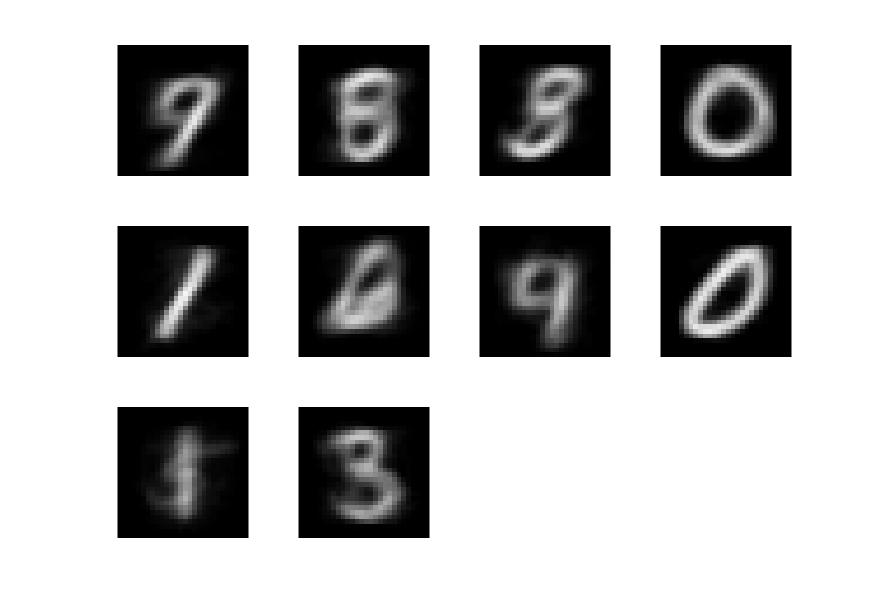
\includegraphics[width=\textwidth]{./56.png}
  \caption{}
  \label{opg56}
\end{figure}
\subsection*{(7)}
We check the coherence of each cluster and find the weighted error, this is found to be:
\[
err = 0.5420
\]
As it can be seen in the visualizations as well as the weighted error, the clustering is not that successful in identifying the digits, it is mostly taking the wrong guess in our case.
\subsection*{(8)}
We want to do a scatter plot of the images with their respective labels shown as shapes and colours, this can be done by applying PCA to the dataset, when this is completed we can plot the first two principle components, this can be seen in figure \ref{opg58}
\begin{figure}[H]
  \centering
  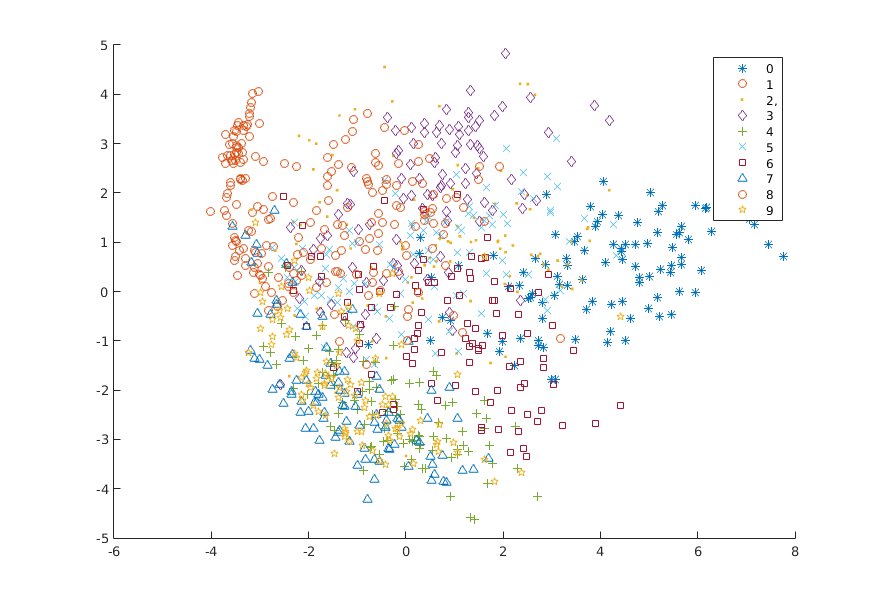
\includegraphics[width=\textwidth]{./58.png}
  \caption{}
  \label{opg58}
\end{figure}
\subsection*{(9)}
We now want to do the same plot as in (7), but this time with the labels according to the centroids for $k=[2,4,8,10,16]$, these plots can be seen in figure \ref{opg59}.
\begin{figure}[H]
  \centering
  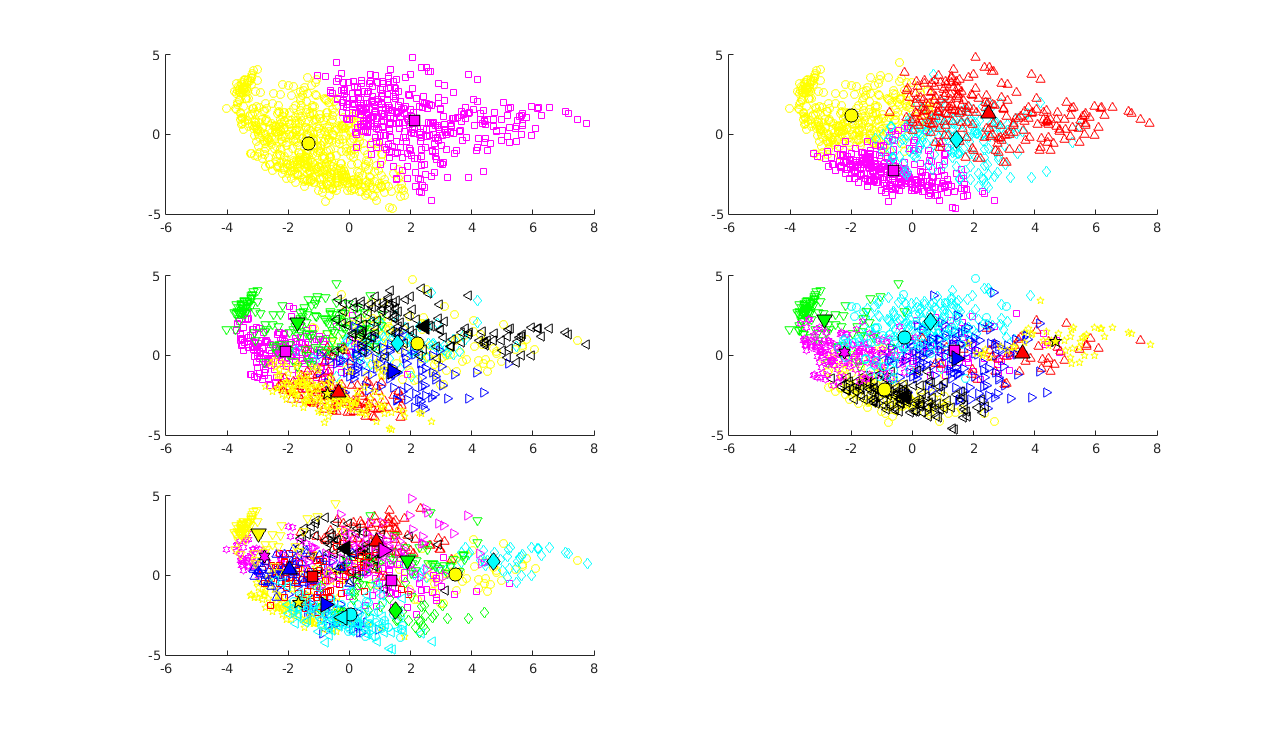
\includegraphics[width=\textwidth]{./59.png}
  \caption{}
  \label{opg59}
\end{figure}

\end{document}